\twocolumn[\colorsection{Distribuciones de carga contínuas}]
\setcounter{figure}{0}

\begin{Exercise}
  Un alambre recto, muy largo, tiene una densidad de carga por unidad de longitud $\lambda = \SI{1.46}{\nano\coulomb/\metre}$. ¿A qué distancia desde el alambre la magnitud del campo eléctrico es $\SI{25.0}{\newton/\coulomb}$?
\end{Exercise}
\begin{Answer}
  $\SI{1.05}{\metre}$
\end{Answer}
%
\begin{Exercise}\label{p:continuas01}
  \textit{a}) Para el segmento mostrado en la figura \ref{f:continuas01}, de longitud $L$ y carga $Q$ distribuida uniformemente, demuestre que el campo eléctrico en el punto $S$ ubicado a una distancia $a$ sobre la mediatriz, está dado por:
  \begin{align*}
    \va*{E} &= \frac{Q}{2\pi\varepsilon_o a} \frac{1}{\sqrt{L^2+4a^2}}\vu{y}
  \end{align*}
  \textit{b}) Para el mismo segmento, demuestre que el campo eléctrico en el punto $P$ vale:
  \begin{align*}
    \va*{E} = \frac{Q}{4\pi\varepsilon_o L} \left \lbrack \frac{1}{b} - \frac{1}{L+b} \right \rbrack \vu{x}
  \end{align*}
  \textit{c}) Si la longitud del segmento es $L = \SI{5.0}{\centi\metre}$ y su carga es $Q = \SI{1.0}{\micro\coulomb}$, calcular la fuerza sobre una carga puntual de $\SI{3.0}{\micro\coulomb}$ si se la ubica en el punto $P$, a una distancia $b = \SI{2.0}{\centi\metre}$.
\end{Exercise}
\begin{Answer}
  \textit{c}) $\va*{F} = \SI{19.3}{\newton}\vu{x}$
\end{Answer}
%
\begin{center}
\begin{tikzpicture}[scale=0.5]
  \draw (0,0) ellipse (0.1 and 0.2);
  \draw (-5,0) +(90:0.1 and 0.2) arc (90:270:0.1 and 0.2);
  \draw [black] (-5,0.2)--(0,0.2);
  \draw [black] (-5,-0.2)--(0,-0.2);
  \draw [blue, dotted] (0,0)--(5,0);
  \draw [blue, dotted] (-7,0)--(-5.1,0);
  \draw [blue, dotted] (-2.5,0.2)--(-2.5,4);
  \draw [blue, dotted] (-2.5,-0.2)--(-2.5,-2);
  \draw [black, -{Stealth}] (-12,0)--(-8,0) node[below] {$x$};
  \draw [black, -{Stealth}] (-11,-1)--(-11,3.5) node[left] {$y$};
  \draw [blue, {Stealth}-{Stealth}] (-3.5,0.2)--(-3.5,3) node[midway, left] {$a$};
  \draw [blue, {Stealth}-{Stealth}] (0,-1)--(4,-1) node[midway, above] {$b$};
  \fill [blue](4,0) circle(5pt) node[above right] {$P$};
  \fill [blue](-2.5,3) circle(5pt) node[above right] {$S$};
\end{tikzpicture}
\captionof{figure}{Problema \ref{p:continuas01}\label{f:continuas01}}
\end{center}
%
\begin{Exercise}
  Una carga neta de $\SI{2.00}{\nano\coulomb}$ está distribuida de manera uniforme a lo largo del eje $y$ entre $y = 0$ e $y = \SI{15}{\centi\metre}$, y una carga puntual de $\SI{-2.00}{\nano\coulomb}$ se encuentra sobre el eje $x$ en la posición $x = \SI{3}{\centi\metre}$. Obtener el vector campo eléctrico resultante sobre el eje $y$, en la posición $y = \SI{-4}{\centi\metre}$.
\end{Exercise}
\begin{Answer}
  $\va*{E} = \SI{4320}{\newton/\coulomb}\vu{x} + \SI{3390}{\newton/\coulomb}\vu{y}$
\end{Answer}
%
\begin{Exercise}\label{p:continuas02}
  Dos varillas delgadas de longitud $L = \SI{3.00}{\centi\metre}$ están a lo largo del eje $x$ como se muestra en la figura \ref{f:continuas02}. Cada varilla tiene carga igual a $\SI{5.00}{\micro\coulomb}$ distribuida de manera uniforme en toda su longitud. Calcular el módulo de la fuerza que ejerce una varilla sobre la otra.
\end{Exercise}
\begin{Answer}
  $\SI{50.7}{\newton}$
\end{Answer}
%
\begin{center}
  \begin{tikzpicture}[scale=0.5]
    \draw (5,0) ellipse (0.1 and 0.2);
    \draw (2,0) +(90:0.1 and 0.2) arc (90:270:0.1 and 0.2);
    \draw [black] (2,0.2)--(5,0.2);
    \draw [black] (2,-0.2)--(5,-0.2);
    \draw (-2,0) ellipse (0.1 and 0.2);
    \draw (-5,0) +(90:0.1 and 0.2) arc (90:270:0.1 and 0.2);
    \draw [black] (-5,-0.2)--(-2,-0.2);
    \draw [black] (-5,0.2)--(-2,0.2);
    \draw [blue, dotted, -{Stealth}] (-7,-0.7)--(7,-0.7) node[below] {$x$};
    \draw [blue] (-5,-0.5)--(-5,-0.9) node[below] {$-5$};
    \draw [blue] (-2,-0.5)--(-2,-0.9) node[below] {$-2$};
    \draw [blue] (0,-0.5)--(0,-0.9) node[below] {$0$};
    \draw [blue] (2,-0.5)--(2,-0.9) node[below] {$2$};
    \draw [blue] (5,-0.5)--(5,-0.9) node[below] {$5$};
  \end{tikzpicture}
  \captionof{figure}{Problema \ref{p:continuas02}\label{f:continuas02}}
\end{center}
%
\begin{Exercise}\label{p:continuas03}
Se tienen dos hilos infinitos con densidad lineal de carga uniforme, ubicados como muestra la figura \ref{f:continuas03}. Uno de los hilos se prolonga a lo largo del eje $y$ ($x=0$) y tiene densidad de carga $\lambda_1 = \SI{-30}{\micro\coulomb/\metre}$, y el otro hilo se encuentra a una distancia $b = \SI{20}{\centi\metre}$ medida sobre el eje $x$, y su densidad de carga es $\lambda_2 = \SI{10}{\micro\coulomb/\metre}$. ¿En qué posiciones sobre el eje $x$ se puede ubicar una carga puntual positiva si se desea que la fuerza neta sobre dicha carga esté dirigida hacia el sentido positivo de $x$?
\end{Exercise}
\begin{Answer}
  \begin{minipage}[t]{.4\textwidth}
  La carga puede estar en $ x < \SI{0}{\centi\metre}$, en $\SI{15}{\centi\metre} < x < \SI{20}{\centi\metre}$,\\ o en $\SI{20}{\centi\metre} < x < \SI{30}{\centi\metre}$
  \end{minipage}
\end{Answer}
%
\begin{center}
  \begin{tikzpicture}[scale=0.5]
    \draw (0,3.5) ellipse (0.2 and 0.1);
    \draw (0,-1.5) +(180:0.2 and 0.1) arc (180:360:0.2 and 0.1);
    \draw [black] (-0.2,-1.5)--(-0.2,3.5) node[midway, left] {$\lambda_1$};
    \draw [black] (0.2,-1.5)--(0.2,3.5);
    \draw (2,3.5) ellipse (0.2 and 0.1);
    \draw (2,-1.5) +(180:0.2 and 0.1) arc (180:360:0.2 and 0.1);
    \draw [black] (1.8,-1.5)--(1.8,3.5);
    \draw [black] (2.2,-1.5)--(2.2,3.5) node[midway, right] {$\lambda_2$};
    \draw [blue, -{latex}] (2.2,0)--(5,0) node[below] {$x$};
    \draw [blue] (0.2,0)--(1.8,0);
    \draw [blue] (-2,0)--(-0.2,0);
    \draw [blue, -{latex}] (0,3.5)--(0,4.5) node[left] {$y$};
    \draw [blue] (0,-2.5)--(0,-1.6);
    \draw [blue, {latex}-{latex}] (0.05,-2)--(1.95,-2) node[midway, above] {$b$};
  \end{tikzpicture}
  \captionof{figure}{Problema \ref{p:continuas03}\label{f:continuas03}}
\end{center}
%
\begin{Exercise}
  Calcular la energía cinética de un electrón que gira en una trayectoria circular alrededor de un hilo infinito con densidad de carga $\lambda = \SI{3E-8}{\coulomb/\metre}$.
\end{Exercise}
\begin{Answer}
  $\SI{4.32E-17}{\joule}$
\end{Answer}
%
\begin{Exercise}\label{p:continuas04}
  \textit{a}) Para el disco mostrado en la figura \ref{f:continuas04}, cuyo radio es $R$ y está cargado con una densidad de carga superficial $\sigma$ uniforme, demuestre que el campo eléctrico producido en el punto $P$ es:
  \begin{align*}
    \va*{E} &= \frac{\sigma}{2\varepsilon_o} \left [ 1 - \frac{z}{\sqrt{z^2+R^2}} \right ] \vu{k}
  \end{align*}
  \textit{b}) Sea la carga neta que se distribuye uniformemente en la superficie del disco igual a $\SI{-6.50}{\nano\coulomb}$ y su radio $R = \SI{1.25}{\centi\metre}$, calcular el campo eléctrico que produce este disco en el punto $P$ a una distancia $z = \SI{2.00}{\centi\metre}$ desde su centro. \textit{c}) Con los mismos valores del ítem \textit{b}, calcular el campo eléctrico en el punto $P$ suponiendo que toda la carga se distribuyera uniformemente en el perímetro del disco.
\end{Exercise}
\begin{Answer}
  \begin{minipage}[t]{.4\textwidth}
    \textit{b}) $\va*{E} = \SI{-1.14E5}{\newton/\coulomb}\vu{k}$\\ \textit{c}) $\va*{E} = \SI{-8.91E4}{\newton/\coulomb}\vu{k}$
  \end{minipage}
\end{Answer}
%
\begin{center}
  \tdplotsetmaincoords{70}{110}
  \begin{tikzpicture}[tdplot_main_coords, scale=0.5]
    %Axis
    \filldraw[fill=red, opacity=0.2,tdplot_main_coords] (4,0,0) arc (0:360:4);
    \draw[axis] (0,0,0) -- (6,0,0) node [pos=1.1] {$i$};
    \draw[axis] (0,0,0) -- (0,6,0) node [pos=1.05] {$j$};
    \draw[axis] (0,0,0) -- (0,0,5.5)  node [left] {$k$};
    \fill [black](0,0,4) circle(3pt) node[left] {$P = (0,0,z)$};
  \end{tikzpicture}
  \captionof{figure}{Problema \ref{p:continuas04}\label{f:continuas04}}
\end{center}
%
\begin{Exercise}\label{p:continuas05}
  El anillo mostrado en la figura \ref{f:continuas05} tiene un radio de $\SI{2.50}{\centi\metre}$ y una carga total igual $\SI{0.125}{\nano\coulomb}$ distribuida uniformemente. El centro del anillo está en el origen de coordenadas. Una carga puntual $q = \SI{-2.50}{\micro\coulomb}$ se coloca sobre el eje $k$ a una altura $b = \SI{40.0}{\centi\metre}$. ¿Cuál es la fuerza ejercida sobre el anillo debida a la carga $q$?
\end{Exercise}
\begin{Answer}
  $\va*{F} = \SI{1.74E-5}{\newton}\vu{k}$
\end{Answer}
%
\begin{center}
  \tdplotsetmaincoords{70}{110}
  \begin{tikzpicture}[tdplot_main_coords, scale=0.5]
    %Axis
    \draw[thick, tdplot_main_coords] (4,0,0) arc (0:360:4);
    \draw[axis] (0,0,0) -- (6,0,0) node [pos=1.1] {$i$};
    \draw[axis] (0,0,0) -- (0,6,0) node [pos=1.05] {$j$};
    \draw[axis] (0,0,0) -- (0,0,5.5)  node [left] {$k$};
    \fill [black](0,0,4) circle(4pt) node[right] {$q$};
    \draw[blue, {Stealth}-{Stealth}] (0.5,-0.5,0) -- (0.5,-0.5,4) node[midway, left] {$b$};
  \end{tikzpicture}
  \captionof{figure}{Problema \ref{p:continuas05}\label{f:continuas05}}
\end{center}
%
\begin{Exercise}\label{p:continuas06}
  \textit{a}) Una carga de $\SI{-12.0}{\nano\coulomb}$ está distribuida de manera uniforme en un cuarto de círculo de radio $a = \SI{25.0}{\centi\metre}$ que se encuentra en el primer cuadrante, con el centro de curvatura en el origen, como se muestra en la figura \ref{f:continuas06}. Calcular el campo eléctrico en el origen. \textit{b}) Encontrar el campo eléctrico en el centro de la semicircunferencia de radio $R$ y densidad de carga lineal uniforme $\lambda$ mostrada en la figura \ref{f:continuas07}.
\end{Exercise}
\begin{Answer}
  \begin{minipage}[t]{.4\textwidth}
    \textit{a}) $|\va*{E}| = \SI{432}{\newton/\coulomb}$; $\theta = 45^\circ$\\ \textit{b}) $\va*{E} = \dfrac{\lambda}{2\pi\varepsilon_o R}\vu{x}$
  \end{minipage}
\end{Answer}
%
\begin{center}
  \begin{tikzpicture}[scale=0.6]
    \draw [very thick] (3,0) arc (0:90:3);
    \draw [blue, -{latex}] (0,0)--(2.12,2.12) node[midway, above] {$a$};
    \draw [blue, -{latex}] (0,-2)--(0,4) node[left] {$y$};
    \draw [blue, -{latex}] (-2,0)--(4,0) node[below] {$x$};
  \end{tikzpicture}
  \captionof{figure}{Problema \ref{p:continuas06} (\textit{a})\label{f:continuas06}}
\end{center}
%
\begin{center}
  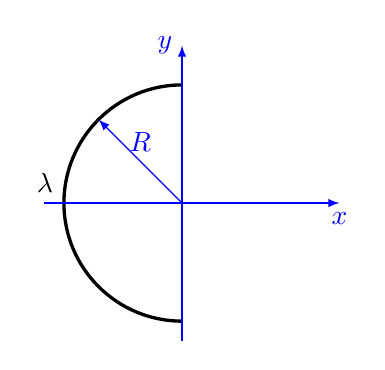
\begin{tikzpicture}[scale=0.5]
    \draw [very thick] (0,3) arc (90:270:3) node[midway, above left] {$\lambda$};
    \draw [blue, -{latex}] (0,0)--(-2.12,2.12) node[midway, above] {$R$};
    \draw [blue, -{latex}] (0,-3.5)--(0,4) node[left] {$y$};
    \draw [blue, -{latex}] (-3.5,0)--(4,0) node[below] {$x$};
  \end{tikzpicture}
  \captionof{figure}{Problema \ref{p:continuas06} (\textit{b})\label{f:continuas07}}
\end{center}
%
\begin{Exercise}\label{p:continuas08}
  Sean dos planos paralelos al plano $yz$, cargados con igual densidad de carga uniforme $\sigma$ y separados por una distancia $a$ como se muestra en la figura \ref{f:continuas08}. Obtener el campo eléctrico en las regiones $x<0$, $0<x<a$ y $a<x$, para puntos alejados de los bordes y cuya distancia al plano sea pequeña comparada con las dimensiones de los planos.
\end{Exercise}
\begin{Answer}
  \begin{minipage}[t]{.4\textwidth}
    $\va*{E}_{x<0} = -\dfrac{\sigma}{\varepsilon_o} \vu{x}$\\ $\va*{E}_{0<x<a} = 0$\\ $\va*{E}_{x>a} = \dfrac{\sigma}{\varepsilon_o} \vu{x}$
  \end{minipage}
\end{Answer}
%
\begin{center}
\tdplotsetmaincoords{70}{110}
\begin{tikzpicture}[tdplot_main_coords, scale=0.5]
	\draw[blue, -{latex}] (2,0,0) -- (6,0,0) node [pos=1.1] {$x$};
	\draw[dotted, blue] (0,0,0) -- (2,0,0);
	\draw[blue, -{latex}] (0,1.35,0) -- (0,4,0) node [pos=1.05] {$y$};
	\draw[blue, dotted] (0,0,0) -- (0,1.3,0);
	\draw[blue, -{latex}] (0,0,2.25) -- (0,0,4)  node [left] {$z$};
	\draw[blue, dotted] (0,0,0) -- (0,0,2.2);
	\draw[blue, {latex}-{latex}] (2,-2.1,3.1) -- (0,-2.1,3.1) node [midway, above left] {$a$};
	\draw[opacity=0.4, tdplot_main_coords] (0,-2,2.25) -- (0,-2,3) -- (0,2,3) -- (0,2,-3) -- (0,1.3,-3);
	\fill[red, opacity=0.4, tdplot_main_coords] (0,-2,2.25) -- (0,-2,3) -- (0,2,3) -- (0,2,-3) -- (0,1.3,-3) -- (0,1.3,2.25) -- (0,-2,2.25);
	\filldraw[fill=red, opacity=0.2, tdplot_main_coords] (2,-2,3) -- (2,2,3) -- (2,2,-3) -- (2,-2,-3) -- (2,-2,3);
\end{tikzpicture}
\captionof{figure}{Problema \ref{p:continuas08}\label{f:continuas08}}
\end{center}
%
\begin{Exercise}
  Dos grandes placas metálicas de $\SI{3}{\metre\squared}$ están colocadas frente a frente, separadas $\SI{5}{\centi\metre}$, y tienen cargas iguales y de signo contrario en sus superficies interiores. Si el módulo del campo eléctrico entre esas placas es $\SI{55E3}{\newton/\coulomb}$, ¿cuál es la carga en cada superficie? (Despreciar efectos de borde.)
\end{Exercise}
\begin{Answer}
  $\pm\SI{1.46}{\micro\coulomb}$
\end{Answer}
%
\begin{Exercise}
  Demuestre que el campo eléctrico fuera de una esfera metálica con una carga eléctrica neta $Q$ es:
  \begin{align*}
    \va*{E}(r) &= \frac{Q}{4\pi\varepsilon_o r^2} \vu{r}
  \end{align*}
  y adentro de la esfera vale $E = 0$.
\end{Exercise}
%
\begin{Exercise}
  El campo eléctrico a una distancia de $\SI{0.145}{\metre}$ de la superficie de una esfera sólida no conductora, con radio de $\SI{0.355}{\metre}$, es de $\SI{1750}{\newton/\coulomb}$. \textit{a}) Suponiendo que la carga se distribuye uniformemente en todo el volumen de la esfera, ¿cuál es la densidad de carga en su interior? \textit{b}) Calcular el campo eléctrico dentro de la esfera a una distancia de $\SI{0.200}{\metre}$ del centro. \textit{c}) Calcular el módulo de la fuerza que ejerce esta esfera sobre una carga puntual de $\SI{25}{\milli\coulomb}$ ubicada a una distancia de $\SI{0.55}{\metre}$ del centro de la esfera.
\end{Exercise}
\begin{Answer}
  \begin{minipage}[t]{.4\textwidth}
    \textit{a}) $\SI{260}{\nano\coulomb/\metre\cubed}$\\ \textit{b}) $\va*{E}=\SI{1960}{\newton/\coulomb}\vu{r}$\\ \textit{c}) $\SI{36.2}{\newton}$
  \end{minipage}
\end{Answer}
%
\begin{Exercise}
  Una esfera hueca, aislante, tiene un radio interior $a = \SI{2}{\centi\metre}$ y un radio exterior $b = \SI{10}{\centi\metre}$. Dentro del material aislante, la densidad de carga volumétrica está dada por $\rho(r) = \alpha/ r$ , donde $\alpha = \SI{36E-6}{\coulomb/\metre\squared}$. \textit{a}) Encontrar el campo eléctrico en la región $a < r < b$. \textit{b}) Si se coloca una carga puntual en el centro del hueco, ¿qué valor debe tener debe tener esa carga para que el campo eléctrico sea constante en la región $a < r < b$.
\end{Exercise}
\begin{Answer}
  \begin{minipage}[t]{.4\textwidth}
    \textit{a}) $\va*{E} = \dfrac{\alpha}{2\varepsilon_o}\left (1 - \dfrac{a^2}{r^2} \right )\vu{r}$\\ \textit{b}) $\SI{90.4}{\nano\coulomb}$
  \end{minipage}
\end{Answer}
%
\begin{Exercise}
  \textit{a}) Para un conductor cilíndrico de longitud infinita, de radio $R$, y densidad de carga superficial uniforme $\sigma$, verificar que su carga por unidad de longitud $\lambda$ se relaciona con $\sigma$ de la siguiente forma:
  \begin{align*}
    \lambda &= 2\pi\sigma R
  \end{align*}
  \textit{b}) Demostrar que el campo eléctrico producido por el cilindro cargado a una distancia $r > R$ desde su eje es:
  \begin{align*}
    \va*{E} &= \frac{\sigma R}{\varepsilon_o r}\vu{r}
  \end{align*}
  \textit{c}) Verificar que esa expresión del campo eléctrico es equivalente al campo eléctrico que se produciría si toda la carga estuviera distribuida sobre el eje del cilindro.
\end{Exercise}
%
\begin{Exercise}\label{p:continuas09}
  La figura \ref{f:continuas09} muestra la sección transversal de un alambre metálico coaxial con un casco cilíndrico, ambos de longitud infinita. Los campos eléctricos en las posiciones $\va*{r}_a$ y $\va*{r}_b$ son $\va*{E}_a = \SI{2000}{\newton/\coulomb}\vu{r}$ y $\va*{E}_b = \SI{-1000}{\newton/\coulomb}\vu{r}$ respectivamente, y las distancias al centro son $r_a = \SI{10}{\centi\metre}$ y $r_b = \SI{30}{\centi\metre}$. Encontrar las cargas por unidad de longitud tanto del alambre ($\lambda_1$) como del casco cilíndrico ($\lambda_2$).
\end{Exercise}
\begin{Answer}
  \begin{minipage}[t]{.4\textwidth}
    $\lambda_1 = \SI{11.1}{\nano\coulomb/\metre}$\\ $\lambda_2 = \SI{-27.8}{\nano\coulomb/\metre}$
  \end{minipage}
\end{Answer}
%
\begin{center}
  \begin{tikzpicture}[scale=0.5]
    \fill [red, opacity=0.3](0,0) circle(1);
    \draw [pattern=north west lines](0,0) circle(1);
    \draw[fill=red!50,even odd rule]  (0,0) circle (3cm) (0,0) circle (2.5cm);
    \draw[pattern=north east lines,even odd rule]  (0,0) circle (3cm) (0,0) circle (2.5cm);
    \draw [blue, -{latex}] (0,0)--(1.4,1.4) node[left] {$\va*{r}_a$};
    \draw [blue, -{latex}] (0,0)--(3.8,0) node[above] {$\va*{r}_b$};
  \end{tikzpicture}
  \captionof{figure}{Problema \ref{p:continuas09}\label{f:continuas09}}
\end{center}
